\subsection{Stability}
\label{subsec:stability}

Stability, when referring to a clock source, is the measure of how well the reference frequency can be maintained over time.
All the metrics used to define the stability of a clock are based on the fractional frequency error, which is the ratio between the frequency error and the reference frequency, namely:

\begin{equation}
  y(t) = \frac{f(t) - f_0}{f_0}
  \label{eq:fractional_frequency_error}
\end{equation}
%
where $f(t)$ is the frequency of the clock at time $t$, and $f_0$ is the nominal frequency of the clock.

In the framework of \acrshort{csacs}, or more in general of atomic clocks, three main regions can be identified in the stability plot: short-term, medium-term, and long-term stability.

\begin{figure}
  \centering
  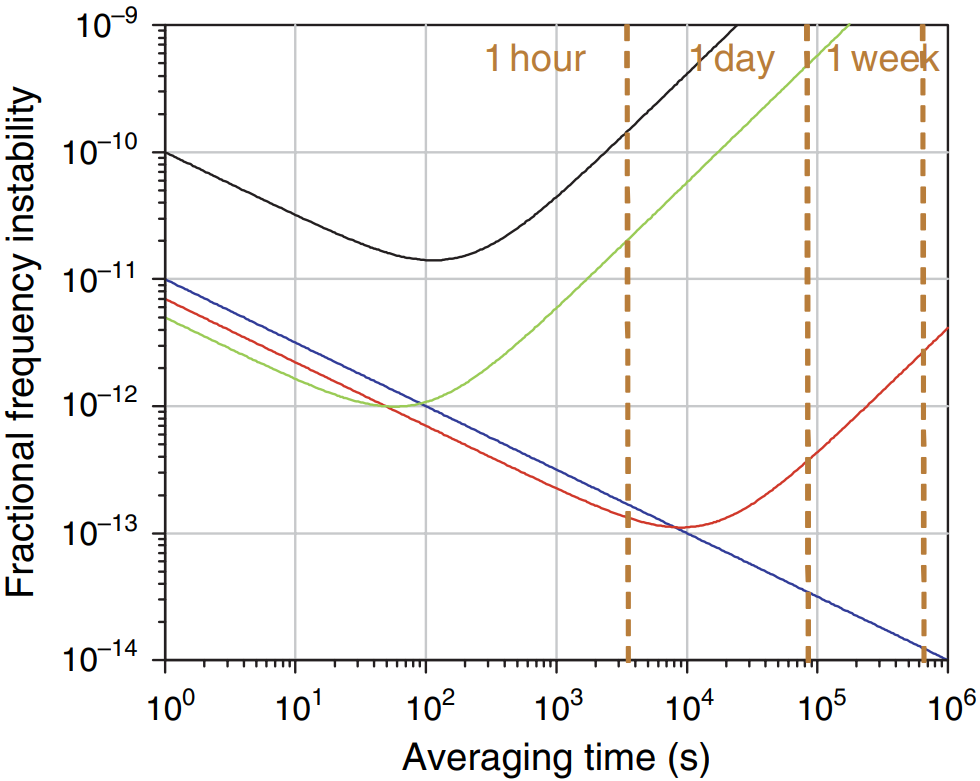
\includegraphics[width=0.6\textwidth, max width=\linewidth]{img/allan-deviation-graph.png}
  \caption{
    Allan deviation plot $\sigma_y(\tau)$ for different clock type sources
    (
    \textcolor[HTML]{0000FF}{\acrfull{cs} Beam Standard},
    \textcolor[HTML]{FF0000}{\acrfull{rb} vapor cell clock},
    \textcolor[HTML]{00FF00}{Oven-controlled crystal oscillator (OCXO)},
    \textcolor[HTML]{000000}{Temperature-compensated crystal oscillator (TCXO)}
    ).
  }
  \label{fig:allan_deviation_graph}
\end{figure}


\subsubsection{Short-term stability}

Short-term stability refers to the performance of a clock over very short time intervals, typically ranging from a few milliseconds to a few minutes.
Allan deviation (denoted as $\sigma_y(\tau)$) is the metric used to measure this, capturing both rapid fluctuations (Fast Noise) and gradual drifts (Slow Drift) in the output frequency.
From its definition, the Allan deviation can be computed as:

\begin{equation}
  \sigma_y(\tau) = \sqrt{\frac{1}{2M} \sum_{i=2}^{M} (\bar{y}(\tau)_{i} - \bar{y}(\tau)_{i-1})^2}
  \label{eq:allan_deviation_short}
\end{equation}
%
where $\bar{y}(\tau)_{i}$ is the average fractional frequency error over the time interval $\tau$ and $M$ is the number of observations.

To give a more practical example, we can consider a clock running with an output frequency of $f_0 = 10MHz$, having an Allan deviation of $\sigma_y(\tau=1s) = 3 \times 10^{-9}$.
In this case, the instability in frequency between two observations 1 second apart has an RMS value of $3 \times 10^{-9}$, that means a $10MHz * 3 \times 10^{-9} = 30mHz$ RMS movement in frequency mostly due to the Fast Noise.

As we will see in Section \ref{sec:working_principles}, for a \acrshort{csacs} clock the component having a major impact on the Fast Noise is the \acrfull{lo}.


\subsubsection{Medium-term stability}

Medium-term stability refers to the performance of a clock over longer time intervals, typically ranging from a few minutes to a few days.
Allan deviation is again the metric used to measure this.
In this case however, knowing that the Slow Drift is the main source of instability, the Allan deviation can be computed using an approximated version of Equation \ref{eq:allan_deviation_short}:

\begin{equation}
  \sigma_y(\tau) = \frac{1}{Q \times SNR} \tau^{-1/2}
  \label{eq:allan_deviation_medium}
\end{equation}
%
where $Q = \frac{\nu_0}{\Delta \nu}$ and $SNR = \frac{P_{signal}}{P_{noise}}$ are related to the quality of the output signal in terms of frequency and power.

This simplified version of the Allan deviation can be adopted after the flicker floor, which is the point where the Fast Noise is no longer the main source of instability, and the Slow Drift becomes the dominant factor.
On a $\sigma_y(\tau)$ plot, the flicker floor can be identified as the point where the Allan deviation reaches a minimum value and then starts to increase again.

As we will see in Section \ref{sec:working_principles}, for a \acrshort{csacs} clock, the cause of the medium-term stability cannot be brought back to a single component, but it's the result of multiple and concurrent effects.


\subsubsection{Long-term stability}

Long-term stability refers to the performance of a clock over very long time intervals, typically ranging from a few weeks to a few years.
Fractional frequency error is the metric used to measure this, and it's computed from the definition given in Equation \ref{eq:fractional_frequency_error}.

In this case, multiple factors can influence this metric, such as aging, environmental conditions, and other external factors.
The summation of all these factors is usually referred to as the Drift, which is the main source of instability in the long-term stability of a clock.

